% !TEX root = ../thesis.tex
% !TeX spellcheck = en_US

% visibility graphs contain shortest paths
% adding source/destination nodes to graph and connecting them allows determination of shortest path between arbitrary locations in the presence of obstacles in the plain
% Connecting visibility edges to roads enables more flexible and realistic routes
% A* routing still fast (speedup methods can be applied) but connecting locations is slowing routing down
This thesis presented a routing algorithm that combines graph-based with geometric routing and was therefore called \emph{hybrid routing algorithm}.
It uses road data as well as open spaces between obstacles to find shortest path.

The geometric routing component is based on visibility graphs, which is a graph that contains only edges between vertices that are visible to each other, i.e. only edges that so not intersect any obstacle from the input dataset.
Edges in visibility graphs are therefore shortest paths between their vertices, which is a useful property for finding general shortest paths between vertices.
Generating a routable visibility graph is one core task of the hybrid routing algorithm.

Merging the visibility graph with the existing road edges from the input dataset is the second core task of the hybrid routing algorithm.
The challenge in this task is the connecting between a road edge and intersecting visibility edges to allow a graph-based routing algorithm to switch between these two types of edges.

The graph-based routing component consists of the popular A* algorithm, but any graph-based routing algorithm, including ones using speedup techniques, could be used.
Because source and destination coordinates of a routing query do not necessarily correspond to vertices in the routing graph, these location must be added to the graph.
After adding vertices for the source and destination, these two new vertices need to be connected to the surrounding graph in order to be reachable by the graph-based routing algorithm.

The evaluation showed expected results for the three main considerations regarding performance and route quality.
First, the overall performance has a quadratic time complexity due to the visibility graph creation, which is inherently quadratic in the number of input vertices.
Second, the route quality does benefit from the presence of open spaces and the routes did become shorter and more realistic with respect to expected routes real pedestrians would likely choose.
This increased realism of the routes therefore can have beneficial effects on agent-based models used to simulate human behaviors.
In contrast to the hybrid routing algorithm, purely graph-based routes showed a lower quality with longer routes and large detours, which is especially the case in rural areas with larger open spaces and a less dense road networks.
And third, the data quality has significant impact on the route quality.
Missing or wrong data might lead to routes, which are not possible in the real world.

However, the presented algorithm has drawbacks which are covered in the following section about potential \hyperref[sec:future-work]{future work} as well as in my following final thoughts on the algorithm.
The most prominent drawback and disadvantage compared to common graph-based algorithm is the low performance.
On the one hand, the visibility graph creation has a quadratic runtime complexity, on the other hand does the implementation still offer potential for performance enhancements.
This concerns both the import and the routing, since new edges might get generated for the source an destination location.
Even though the generated hybrid visibility graph can be stored to disk and only needs to be created once, the routing time cannot be optimized by such simple caching and precomputation.
Depending on the agent-based model, this might significantly increase the simulation time.
Additional problems and concerns are discussed in the section below.

However, I am convinced, that use-cases in agent-based simulations as well as real-world applications exist where the benefits of the hybrid routing algorithm outweigh its drawbacks.

\section{Future work}
\label{sec:future-work}

	This sections discusses known problems with the presented hybrid routing algorithm including potential solutions, potential technical enhancements to the implementation as well as beneficial functionalities.

	\subsection{Known problems}
		% Overall: Speed up visibility edge generation for initial import + routing
		Even though it might not be a severe problem, the graph generation and routing performance offers potential to be improved, either by an optimization of the current implementation or by implementing a different graph generation algorithm.
		
		\begin{wrapfigure}{r}{0.35\textwidth}
			\vspace{-1.5\baselineskip}
			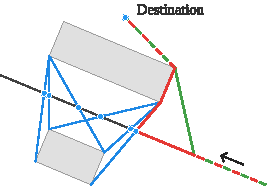
\includegraphics[width=\linewidth]{images/qgis-future-work-connectivity-problem}
			\caption{Connectivity problem in case of too few visibility edges. The green path might be the expected result but the red path is the actual shortest path.}
			\label{fig:connectivity-problem}
			\vspace{\baselineskip}
			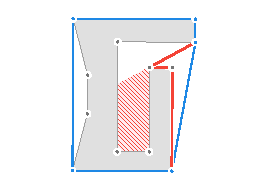
\includegraphics[width=\linewidth]{images/qgis-future-work-convex-hull-problem}
			\caption{Concave polygons do not always contain all necessary edges (red) but only those edges connecting the convex hull (blue). Some regions are therefore unreachable (red marked area).}
			\label{fig:convex-hull-problem}
		\end{wrapfigure}
		
		The first approach might use better data structured for vertices and obstacles.
		In the current implementation, for every vertex, ever other vertex in the dataset is considered a potential neighbor and then filtered out using e.g. valid angle and shadow areas.
		Using a QuadTree might increase performance for this process since not all vertices need to be checked.
		However, any additional data structure also introduces additional overhead and might only be beneficial for datasets of a certain size.
		The usefulness of this approach needs testing and evaluation.
		
		The second approach to reduce graph generation times is a complete reimplementation of the edge creation.
		Such a reimplementation might use approaches mentioned in \Cref{subsec:suitablilty-edge-creation-approaches}, which showed promising sub-quadratic runtime complexities.
				
		% Connection to roads based on the hope that there are many visibility edges (in the end the vast number of edges creates a irregular grid like structure even though v-edges are not connected to each other)
		A problem that might arise with datasets containing very few obstacles are the reduced possibilities to leave a road in order to traverse an open space.
		This is illustrated in \Cref{fig:connectivity-problem} where the green expected path cannot be used due to missing edges.
		Forcing the creation of additional edges, i.e. by connecting all vertices of roads and maybe even creating new vertices by splitting roads at certain distances.
		
		Another known problem arises with islands inside of obstacles, for example an island inside a lake that is reachable via a road edge.
		Even though the hybrid routing algorithm does create edges inside the island, it may also create edges inside the lake.
		Handling inner rings of (multi-)polygons is therefore needed to correctly navigate within islands of obstacles.
		
		% Convex hull filtering might lead to problems for obstacle part not directly visible to outside (like a cave). Concave hull filtering might be the correct solution.
		One optimization of the graph generation process is the filtering of vertices by convex hull as introduced in \Cref{subsubsec:convex-hull}.
		This optimization, however, only works for polygons with no hidden vertices, i.e. vertices with are theoretically reachable but inside the obstacle and not visible to the outside.
		\Cref{fig:convex-hull-problem} illustrates the problem with the red marked area, which is not reachable when only vertices of the convex hull are connected.
		The red edges are necessary to reach every location in- and outside the obstacle.
		
		% Taking road restrictions into account (tags as well as size)
		% Point like barriers (e.g gate on a road) have nearly no effect → generate orthogonal line-barrier or remove all visibility edges within a radius or something
		
	\subsection{Technical enhancements}
		% kD-tree implementations: MARS implementation expensive, NTS implementation only works on classes (MARS stuff often struct) + not supports multiple nodes at same location. Own implementation specifically for points might help
		% Splitting vertices by their valid angle area might simplify implementation + speeds up graph generation since angle area checks are very very fast.

	\subsection{Additional functionalities}	
	% Features:
		% 3D data: Handling OSM level-tags (vertical relation between roads)
		% Storing graph in a format that keeps the same-location-nodes + additional angle information
		% Parallel usage of routing
		% Adding attributes to edges (e.g. when visibility edge goes over grass area → surface=grass to edge)
		% Connecting visibility egdes to each other might be a good idea when adding attributes to the edges
		% Reduce edge-count e.g. with approaches described in "A Modular Routing Graph Generation Method for Pedestrian Simulation" (Kielar, 2016). This might not speed up anything, though since the visibility calculation is based on vertices. However, this might result in fewer road-segments and faster connection of new edges (which is not that slow anyway)
		% Dynamic changes in obstacles, meaning add, remove or change existing obstacles. Visibility edges need to be re-calculated, but not all → which ones?